\documentclass[conference]{IEEEtran}
\IEEEoverridecommandlockouts
% The preceding line is only needed to identify funding in the first footnote. If that is unneeded, please comment it out.
\usepackage{minted}
\usepackage{cite}
\usepackage{amsmath,amssymb,amsfonts}
\usepackage{algorithmic}
\usepackage{graphicx}
\usepackage{textcomp}
\usepackage{xcolor}

\def\BibTeX{{\rm B\kern-.05em{\sc i\kern-.025em b}\kern-.08em
    T\kern-.1667em\lower.7ex\hbox{E}\kern-.125emX}}
\begin{document}

\title{PAVE: An In Situ Framework for Scientific Visualization and Machine Learning Coupling\\
}

\author{\IEEEauthorblockN{1\textsuperscript{st} Samuel Leventhal}
\IEEEauthorblockA{\textit{University of Utah School of Computing} \\
\textit{Scientific Computing and Imaging Institute}\\
Salt Lake City, UT., USA \\
samlev@cs.utah.edu}
\and
\IEEEauthorblockN{2\textsuperscript{nd} Mark Kim}
\IEEEauthorblockA{\textit{Oak Ridge National Laboratory} \\
Oak Ridge TN., USA \\
kimmb@ornl.gov}
\and
\IEEEauthorblockN{3\textsuperscript{rd} David Pugmire}
\IEEEauthorblockA{\textit{Oak Ridge National Laboratory} \\
Oak Ridge TN., USA \\
pugmire@ornl.gov}
}

\maketitle

\begin{abstract}
    The need for researchers and practitioners to have access to {\it in situ} operations is increasing for artificial intelligence and visualisations tasks as implementations become more complex and scaled widening the gap between computation time and IO throughput. What is more, a growing number of applications continue to be developed dealing with the combination of these two domains. With PAVE we present a solution which allows in place data management between visualisation and machine learning tasks. We then demonstrate our framework with the application of a conditional Generative Adversarial neural Network (cGAN) capable of in situ and at scale training over path traced images resulting in a generative model able to produce real-time scene renderings with accurate light transport and global illumination of a quality comparable to offline approaches. 
    
\end{abstract}

\begin{IEEEkeywords}
    VTKm, neural networks, generative adversarial network, in-situ, PyTorch, path tracing
\end{IEEEkeywords}


% \begin{teaserfigure}
%     \includegraphics[width=\textwidth]{buffer_results_teaser.png}
%     \caption{\textmd{Rendered Conditional Geometry Buffers ({\bf left set}) and artificial rendering with conditional generative adversarial neural network ({\bf right couple}) comparing ground truth path traced rendering ({\bf left}) with image generated ({\bf right}).}}
%     \Description{Conditional Buffers and path traced rendered with VTKm to be used for training a PyTorch conditional generative adversarial network.}
%     \label{teaser}
%   \end{teaserfigure}
\section{Introduction}
As IO bandwidth continues to be significantly less than compute, in-situ frameworks have become essential in the modern HPC environment. Further, machine learning (ML) has become a signficant driving force within the HPC community, particularly to help analyze this ever increasing amounts of data. However, machine learning is predicated on the notion that programs or algorithms are constructed by combining data with output, which is the inverse of traditional programming: data and an algorithm generate output (Fig.~\ref{fig:ml-vs-trad}). Therefore, resources must be utilized to develop machine learning algorithms. 

To generate sophisticated machine learning algorithms often requires a significant amount of computation as well as copious amounts of output as input. The purpose of this project is then to offer a solution which provides the means necessary to design machine learning implementations at scale and in situ to aid or be the basis of scientific visualisation tasks. We accomplish this by providing read, write and in place data transfer functionality between learning models and visualisation task implementations. To our knowledge, this is the first scientific visualization-machine learning in-situ framework.

\begin{figure}
    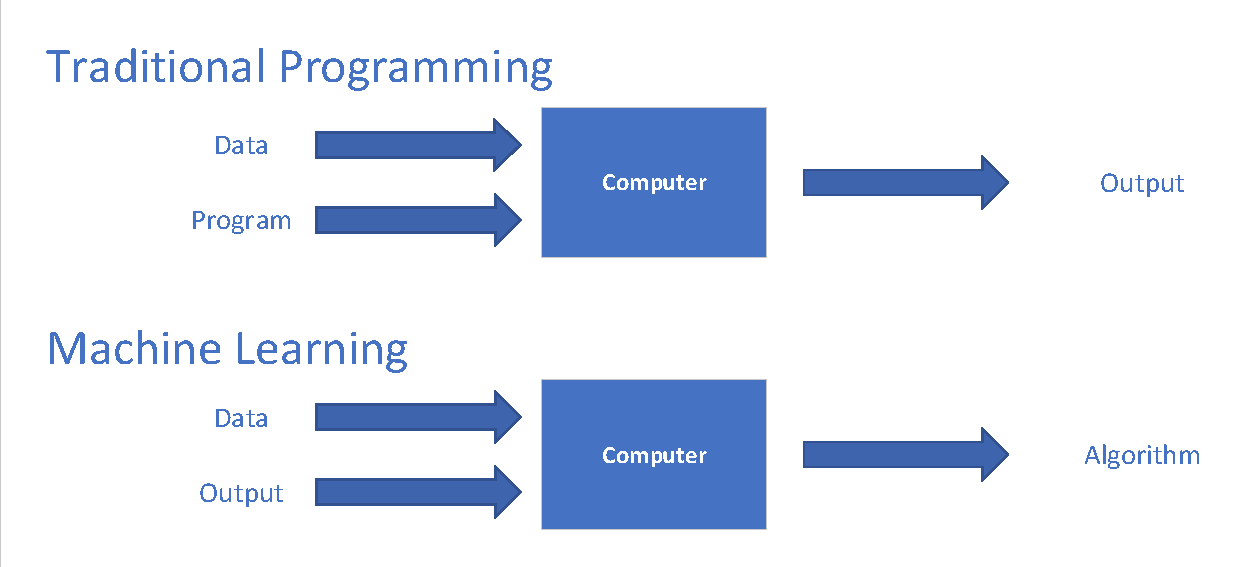
\includegraphics[width=\linewidth]{ML-data-output-program}
    \caption{Traditional programming vs machine learning.}
    \label{fig:ml-vs-trad}
  \end{figure}

In this work we present PAVE, an in-situ framework for coupling scientific visualization and machine learning along with a case study of coupling a path tracer, an accurate light transport simulation, with a neural network to build a filter for real time rendering and accurate light transport. The provided model is a coalescence of the Visualisation Toolkit fit for Massively threaded architectures (VTK-m) and Python, an increasingly popular language within the machine learning community due to robust libraries available for neural networks such as PyTorch. The resulting work accomplishes this combination by utilising VTK-m to construct a path trace rendering tool able to fluidly and efficiently communicate to a cGAN by means of PAVE during training.   The resulting generative model serves as a real-time filter for rendering globally illuminated images which accurately approximate diffuse indirect illumination and soft shadows with quality comparable to offline approaches. 

\begin{figure*}
    \includegraphics[width=\linewidth]{buffer_results_teaser}
    \caption{Rendered Conditional Geometry Buffers ({\bf left set}) and artificial rendering with conditional generative adversarial neural network ({\bf right couple}) comparing ground truth path traced rendering ({\bf left}) with image generated ({\bf right}).}
  \end{figure*}


\section{Related Work}
\subsection{In situ Data Management}
As output sizes of simulations have grown to petabytes of data, new strategies are required to handle the volumes of data generated. In situ analysis and visualization frameworks have emerged to handle this deluge of data, dependent on the needs and requirements of the HPC application~\cite{Abbasi2010, Ayachit:2015:PCE:2828612.2828624,Childs:VisIt-HPV-Chapter:2012, 6846460}. Some frameworks provide a generic data interface~\cite{Ayachit:2016:SGS:3018859.3018867,Larsen:2017:ASI:3144769.3144778} with triggers~\cite{Larsen:2018:FSS:3281464.3281468}. Others focus on in situ, IO-oriented approaches~\cite{doi:10.1002/cpe.3125}, which enables new paradigms for in situ performance~\cite{Kress:ISC19}.

\subsection{Heterogeneous Visualization}
Heterogeneous environments in HPC require new solutions for extracting the most performance. The accelerator, such as GPGPU, in these heterogeneous environments have thousands of concurrent threads with various APIs, such as CUDA~\cite{CUDA} or Thread Building Blocks~\cite{books:daglib:0018624}. Thrust~\cite{hoberock2009thrust} is a proprietary API for parallel primitives programming~\cite{Blelloch:1990:VMD:91254} on Nvidia hardware. VTK-m is a data parallel primitive toolkit for scientific visualization~\cite{vtkm} which has a general parallel programming model with multiple backends to facilitate porting to different heterogeneous systems. 

\subsection{Path Tracing}
Real time, true to life quality renderings of light transport remains an active area of research with a number of various approaches. To preserve real-time rates, previous works have stored precomputed radiance transfers for light transport as spherical functions within a fixed scene geometry which are then adjusted for varied light and camera perspective through projections within a basis of spherical harmonics \cite{sloanPrecompRad}. Similarly, Light Propagation Volumes have been used to iteratively propagate light between consecutive grid positions to emulate single-bounce indirect illumination \cite{kaplanyanCasac}. More recently, deep neural  networks have been employed as a learned look up table for real-time rates with offline quality. With the use of convolutional neural networks Deep Shading is able to translate screen space buffers to into desired screen space effects such as indirect light, depth or motion blur. Similar to the methodology implemented in this work, Deep Illumination uses a conditional adversarial network (cGAN) to train a generative network with screen space buffers allowing for a trained network able to produce accurate global illumination with real-time rates at offline quality through a ``one network for one scene'' setting  \cite{deepillum}.
\section{Coupling Scientific Visualization and Machine Learning}
PAVE is an in situ coupling framework based on ADIOS~\cite{doi:10.1002/cpe.3125}. The resulting framework consists of two core components, visualization output and learning. A scientific visualization application is coupled through the C++ interface, and the output is sent through PAVE to the machine learning application for processing.PAVE then allows each task to communicate results among each other seamlessly. The scientific visualisation task developed by the user can then provide resulting visualisations to a separately developed learning model as input or employ a learning model within the visualisation task.  



\subsection{User Provided Visualisation}

PAVE couples visualization and machine learning through an in situ framework based on ADIOS~\cite{doi:10.1002/cpe.3125}. ADIOS provide a united interface which allows, among other things, memory-to-memory transport between applications during the IO phase of a simulation, i.e. ``in transit in situ.'' With the  unified interface, applications can be coupled either memory-to-memory or through the filesystem. The results for the scalable, in-situ scientific visualization task designed by the user, are passed to a learning model through a single interface and the visualization can remain fully scalable to distributed systems because of PAVE. For this same reason in the provided example in section \ref{ex} we chose VTK-m arrays as the data structures of the visualisation task.

\setminted{fontsize=\footnotesize,baselinestretch=1} 
\begin{listing}[htb]
\noindent\rule{0.5\textwidth}{1pt}
\inputminted{cpp}{pave_pt.py}\label{PAVEvis}
%\inputminted{python}{adiosdataloader.py}
\noindent\rule{0.5\textwidth}{1pt}
\caption{C++ Interface for PAVE}
\label{fig:cpp_interface}
\end{listing}

The interface in Listing~\ref{fig:cpp_interface} demonstrates the visualisation component of PAVE. PAVE is initialized with a name for the dataset that will be used with the machine learning application. As each datum (image, text, etc.) is generated, it is ``saved'' to the dataset. However, PAVE will buffer the data until either an explicit ``flush'' is called, which will flush the current in-memory data to disk, or the dataset is completed. 

\subsection{User Defined Machine Learning Application}

PAVE allows researchers or practitioners to implement their learning algorithms in the increasingly popular language Python due to having a robust library for learning tasks and notably neural networks. 

\begin{listing}[htb]
\noindent\rule{0.5\textwidth}{1pt}\label{PAVElearn}
\inputminted{python}{pave.py}
%\inputminted{python}{adiosdataloader.py}
\noindent\rule{0.5\textwidth}{1pt}
\caption{Python Interface}
\label{fig:python_interface}
\end{listing}

In Listing~\ref{fig:python_interface}, we demonstrate employing PAVE while training a PyTorch model. The training method for Model is able to request visualisation samples used during training based on some parameter used in the visualisation task or retrieve precomputed visualisation data by calling PAVE.
 
\subsection{Communication of Visualisation Data and Learning}

As demonstrated in Section~\ref{PAVEvis} and PAVE allows for the user to save or pass data produced by the simulation and similarly the user would also be able to request results from the learning model depending on the application. Section \ref{PAVElearn} demonstrates PAVE's support in requesting data in place from the user's visualization implementation during training of a predictive model used as example. 

\section{Case Study: Coupled Path Traced Machine Learning}

Utilisation of PAVE consists of three consecutive phases: rendering phase of conditional training images, training phase of the generative neural network, and execution phase of the trained network. Three core components, VTK-m, PyTorch, and PAVE, each fulfill a unique functional requirement during the separate stages. In this section we describe the independent design and global role each system plays.

\subsection{System Overview}
 
To achieve our goal of a conditional generative neural network capable of rendering geometric dependent object path simulations we begin by rendering informative conditional image buffers along with ground truth scene renderings. For this purpose the VTK-m was chosen due to its scalability and robust capability for HPC visualisation tasks. Provided the training set of conditional and ground truth images two neural networks, one convolutional and one generative, play a zero-sum game common to training GANs. To segue data management of training images the path tracer saves the training set in a distributed setting with the use of PAVE. During training PyTorch is then able to retrieve needed image data through the use of the PAVE.

\subsection{Path Tracer Design}

High quality ground truth rendered scenes and conditional image attributes are required for the training stage. For this reason, the first stage of PAVE consists of generating a visual scene or simulation with VTK-m. 

Within the parallel primitives framework of VTK-m, a path tracer was implemented to renders scenes. A path tracer utilizes Monte Carlo sampling through probability distribution functions over shapes of interest and light intensity and pixel values with cumulative distribution function sampling, light scattering, randomly directed light paths and material sampling to generate realistic lighting for a scene. 

Further, the image buffers needed to compute light paths afford an informative conditional dependency on the behavior of lighting based on the geometry and light sources within a scene. The VTK-m ray tracer~\cite{95260c8902184519bd98df42d2572515} was adapted to render these conditional buffers, namely albedo, direct lighting, normals of surfaces and depth with respect to point of view are then stored or passed to PyTorch with PAVE, allowing for a a pipeline which preserves the solutions scalability. 

\subsection{Neural Network Design}

The cGAN used closely follows that introduced by Thomas and Forbes with Deep Illumination \cite{deepillum}. Both the discriminator and generator network are deep convolutional neural networks implemented in PyTorch using training data retrieved from Adios files formatted and stored by the VTK-m path tracer. The training stage relies on four conditional buffers depth, albedo, normals and direct lighting along with an associated ground truth image of high light sample count and ray depth. Given the four conditional buffers the generator attempts to construct the ground truth image from noise. The discriminator is then fed both the generated and ground truth image. The loss used for the gradient back propagation update of both networks is based on the quality of the discriminators ability to classify the artificial and true image in which the generator is greater penalised when the discriminator accurately differentiates the two images, and similarly, the discriminator has a larger loss when incorrectly identifying real from fabricated images. The generator is then considered to have converged when the discriminator predicts both generated and true images with equal probability. For both discriminator and generator networks the activation functions used between layers is LeakyReLu and Sigmoid for the final layer \cite{maasLeaky}. Batch normalisation is also performed between internal layers to minimise covariant shift of weight updates and improve learning for the deeper networks used \cite{ioffeBatch}.

\subsubsection{Generator Network}

The generative network used is a deep convolutional network consisting of an encoder and decoder with skip connections-concatenations of equal depth layers within the encoding and decoding stages. Due to the illustrative `shape' of this design the network is denoted a U-Net as introduced by Ronneberger et. al. for medical segmentation \cite{ronnebergerUnet}. The motivation for utilising a U-Net is due to success of the skip connections in capturing geometric and spatial attributes by linking the decoded convolutional process to the encoded upconvolutional. The mapping of contracting feature segmentation onto expanding upsampling within the network allows us to also exploit nearness to object geometry within the constructed and target image through Euclidean distance. As a result, performance in terms of required training time, quality of preserved structure, and accuracy maintaining light information of generated images drastically improves with the addition of an L1 loss to the classic binary cross entropy common to training adversarial networks when updating the discriminator and generator  \cite{isolaL1}\cite{goodfellowGAN}. 

\subsubsection{Discriminator Network}

For discriminating between artificial and ground truth image renderings a deep convolutional patchGAN network is used motivated by the added advantage of providing a patch-wise probability of an image in question as being real or fake. The benefit of a patch-wise probability allows for higher regional accuracy within an image as well as applicable for image-to-image tasks as introduced by Isola et. al. \cite{isolaPatch}. The image classification probability is then interpreted as the average of these patch wise probabilities over an image in question. 

As input during training the discriminator network is given the set of conditional space buffers along with either the visualisation generated by the cGAN generator network or the ground truth global illumination rendering produced with the VTK-m path tracer. Taking into account the conditional image buffers stacked atop an image sample an image sample under question the resulting input is a tensor of the form Width x Height x 15. The discriminator then attempts to predict with what probability the provided image stack, either fabricated by the U-Net or the VTK-m path tracer, is real. Based on the discriminators performance the loss is computed using the classic loss for training GANs along with an L1 loss. Training is complete, and the generator has converged, when the discriminator predicts images as real or fake with an equal probability, e.g. 50\% chance of accuracy. At this point the discriminator network is discarded and the resulting generator affords a real-time in situ visualisation tool able to produce accurate global illumination from conditional geometric buffers.



\subsection{Our Provided Example of PAVE}\label{ex}

For our PyTorch in situ proposal the current systems we employ are VTK-m, for rendering path traced images and conditional geometry buffers focus, and Adios2 for data management. We discuss the design pattern for our in situ visualisation task with support from deep learning in the order of operations followed within the pipeline of use. Namely, we present the design pattern for rendering light transport in VTK-m coupled with data transport to PyTorch (\ref{pathtracer}). Subsequently we explain the infrastructure for embedding VTK-m throughput managed by Adios2 within PyTorch and demonstrate through example (\ref{pytorch}) by  instantiating a PyTorch data interface allowing for data parallelization and multi-GPU/distributed training as used within the framework for training our cGAN model.

\subsubsection{VTK-m Light Transport Visualisation}\label{pathtracer}

Path traced images are maintained within C++11 as VTK-m arrays which can be passed by reference directly to PyTorch using Adios2 APIs or written to Adios2 .bp file and retrieved during training or when utilising the neural network to generate novel scene renderings from rendered geometry buffers. 

\subsubsection{PyTorch cGAN Global Illumination Generator}\label{pytorch}

For training, our solution used by the cGAN is ``{\it AdiosDataLoader}'', a data class inheriting from the abstract indexing class PyTorch {\it torch.utils.data.Dataset}. The {\it AdiosDataLoader} employs Adios2 to either retrieve from file or have passed by reference vector representations of path traced images and conditional buffers. Within VTK-m during generation these vectors represented as VTK-m vectors and within PyTorch as numpy arrays. In this manner the training or test sets needed by PyTorch and created by VTK-m are available to PyTorch in situ or with reference to written memory. If retrieving VTK-m's renderings PyTorch will compile Adios2 attributes from file as tabled by Adios2 into .bp files. VTK-m generated datasets can be retrieved with {\it read\_adios\_bp()} or passed to a similar {\it get\_adios\_bp()} and subsequently forwarded to our {\it get\_split()}  to partition the dataset into 60\% training, 20\% testing and 20\% validation subsets. The split datasets are then used to construct the {\it AdiosDataLoader} class which inherits from the {\it torch.utils.data.DataLoader} thereby providing a data sampler of our VTK-m renderings with a single-process or multi-process iterator over the dataset affording the tools necessary to train our neural networks in the canonical manner.

% other example scripts
%\inputminted{python}{pytorchAdiosRead.py}
%\inputminted{python}{trainingSplit.py}




In the above code sample the {\it AdiosDataLoader} class is used to partition the data set into training, validation and testing as well as offer a distributable data sampler with an array-like data structure allowing index access to elements and collection size functionality.

%\noindent\rule{0.5\textwidth}{1pt}
%\inputminted{python}{adiosdataloader.py}
%\noindent\rule{0.5\textwidth}{1pt}

\section{Cornell Box Experiment}

To evaluate the quality of in situ deep learning aided visualisations train the cGAN networks on rendered images of a Cornell box, a commonly used 3D modelling framework for quality assessment. We train the model using renderings of the Cornell box with high light sample count and depth computation per ray for various camera angle perspectives into the box along with the associated image geometry buffers for a given camera orientation. We then assess the quality of the models final generated renderings looking at the accuracy of global illumination. We then also demonstrate the performance of the models ability to render global illumination when given image buffers for a novel scene not used for training similar in content but not exact. The scene used for training is comprised of the classic set up with one overhead light source in the center of a white ceiling, a white back wall and a white floor. The remaining walls are then colored red on the left and green on the right in order to afford different colored light transport and demonstrate diffuse interreflection. The contents of the Cornell box are three cuboids of various shapes and sizes to provide diverse shading and diffused lighting. 

%\vspace{-1.5em}
\begin{figure}[h]
\includegraphics[width=0.25\textwidth]{sc-1080-d-45.png}
\end{figure}
%\vspace{-1em}

The conditional differed shading geometry buffers used are direct lighting, normal planes, depth and albedo as shown in figure \ref{teaser}.
\iffalse
\begin{figure}[h]
\caption{\textmd{Global illumination conditional image buffers. {\bf Top:} Albedo, left. Depth, right. {\bf Bottom:} Normals, left. Direct lighting, right.}}
\includegraphics[width=0.40\textwidth]{demo.png}
\label{Gbuf}
\end{figure}
\fi
The geometry buffers serve as joint variables for the conditional probability distribution which the global illumination path traced images are considered to exist. The conditional arguments in this experiment then aid the cGAN in learning behavior of light paths given the geometry of a scene in question. 

\section{Results}
\subsection{Cornell Box Experiment Results}
The resulting generated images show promising results for deep learning aided in situ scientific visualisation. We observe the network successfully learned to emulate light transport in a realistic fashion with offline performance {\bf EXAMPLE}. What is more, though designed in a ``one network for one scene'' setting, the generative net proved to be adaptive and able to generate accurate renderings for not only unobserved camera orientation renderings during training but also varied scenes of a similar flavor when provided the conditional geometry buffers of the novel scene. 
%\vspace{-1.5em}
%\begin{figure}[h]
%\includegraphics[width=0.5\textwidth]{discrimloss.png}
%\end{figure}
%%\vspace{-1em}

%\vspace{-1.5em}
%\begin{figure}[h]
%\includegraphics[width=0.5\textwidth]{genloss.png}
%\end{figure}
%\vspace{-1em}
\subsection{Solution Design Assessment}

To render 3080 256x256 images with the VTK-m path tracer utilizing 2 Nvidia RTX-2080 Ti GPUs required 12 hours. Training the cGAN on this image data set over \_\_\_ epochs on the same machine took \_\_\_ hours. Once trained the run time of applying the generative U-Net provided the conditional buffer set averages \_\_\_ seconds. 

\section{Conclusions}

Our work offers a distributable and scalable implementation and framework to allow researchers and practitioners to easily integrate state of the art deep learning tools afforded by the approachable PyTorch and robust visualisation resource VTK-m for in situ graphics rendering or scientific simulation for HPC systems. With the presented example application utilising cGANs for generative visualisation also offers the prospect of quickly and accurately visualise conditionally dependent data such as light path global illumination's dependence on scene geometry. Subsequently we here then also offer a framework for visualisation within C++ with the use of VTK-m as well as Python in tandem or independently. 


%%
%% The acknowledgments section is defined using the "acks" environment
%% (and NOT an unnumbered section). This ensures the proper
%% identification of the section in the article metadata, and the
%% consistent spelling of the heading.
\section*{Acknowledgment}
 This research was supported in part by an appointment to the Oak Ridge National Laboratory ASTRO Program, sponsored by the U.S. Department of Energy and administered by the Oak Ridge Institute for Science and Education.



\bibliographystyle{IEEEtran}
\bibliography{pave_ref}
\vspace{12pt}
\color{red}
IEEE conference templates contain guidance text for composing and formatting conference papers. Please ensure that all template text is removed from your conference paper prior to submission to the conference. Failure to remove the template text from your paper may result in your paper not being published.

\end{document}
